\selectlanguage{ngerman}

\section{Kernel Optimierungen}

\subsection{Methoden zur Optimierung}
Um die Bootzeit zu optimieren, sollten Kerneländerungen schrittweise vorgenommen und regelmäßig Snapshots
erstellt werden. Dadurch lassen sich Probleme leichter identifizieren und rückgängig machen. Zur Analyse von
Engpässen in der Kernel-Initialisierung bietet sich der Bootparameter \textit{initcall\_debug} an, der die
zeitaufwendigsten Initialisierungsfunktionen auflistet.

\subsection{Kernelkompression}
Die Wahl des Kompressionsalgorithmus hat einen direkten Einfluss auf die Bootzeit. Auf STM32F769NIH6 (dem
Prozessor des STM32F769I-Disco Boards) hat sich Lz4 als die besten Optionen erwiesen, da sie einen guten
Kompromiss zwischen Kompressionsrate und Dekompressionsgeschwindigkeit bieten. Da die Performance stark von
der Zielhardware abhängt, sollten verschiedene Algorithmen getestet werden.

\begin{figure}[ht]
	\centering
	\begin{minipage}{0.48\textwidth}
		\centering
		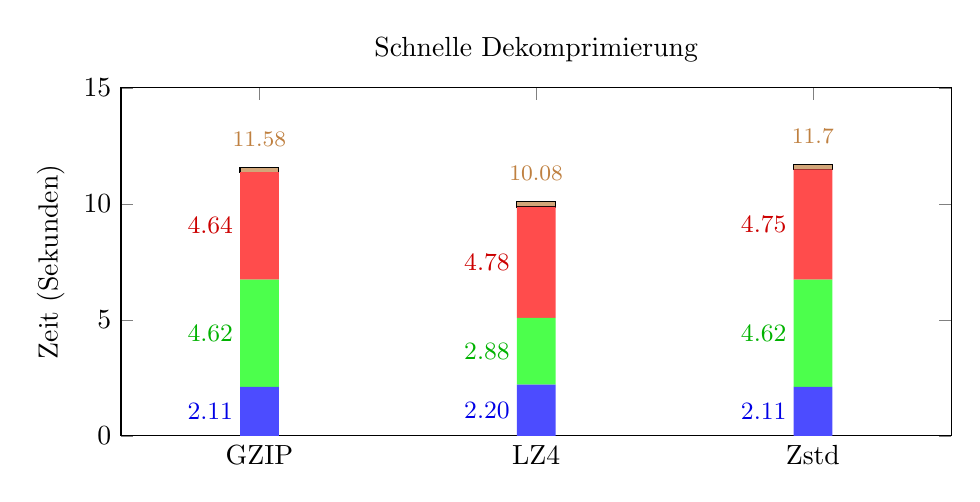
\begin{tikzpicture}
			\begin{axis}[
					ybar stacked,
					bar width=14pt,
					width=\textwidth,
					height=6cm,
					legend style={at={(0.5,-0.25)}, anchor=north,legend columns=-1,font=\small},
					ylabel={Zeit (Sekunden)},
					symbolic x coords={GZIP, LZ4, Zstd},
					xtick=data,
					ymin=0, ymax=15,
					enlarge x limits=0.25,
					title={Schnelle Dekomprimierung},
					nodes near coords,
					nodes near coords style={
							font=\small,
							/pgf/number format/fixed,
							/pgf/number format/precision=2,
							anchor=east,
							xshift=-6pt,
						},
					every node near coord/.append style={
							/pgfplots/point meta=explicit symbolic,
							font=\small,
						},
					point meta=explicit symbolic,
				]
				% U-Boot Time (blue)
				\addplot+[fill=blue!70, draw=none, nodes near coords style={text=blue!90!black}]
				coordinates {(GZIP,2.1124)[2.11] (LZ4,2.2034)[2.20] (Zstd,2.1131)[2.11]};
				% Uncompress Time (green)
				\addplot+[fill=green!70, draw=none, nodes near coords style={text=green!70!black}]
				coordinates {(GZIP,4.6180)[4.62] (LZ4,2.8844)[2.88] (Zstd,4.6180)[4.62]};
				% Kernel Time (red)
				\addplot+[fill=red!70, draw=none, nodes near coords style={text=red!80!black}]
				coordinates {(GZIP,4.6374)[4.64] (LZ4,4.7767)[4.78] (Zstd,4.7541)[4.75]};
				\addplot+[
					fill=brown!70,
					nodes near coords={
							\textbf{\textcolor{brown}{\pgfmathprintnumber[fixed,precision=2]{\pgfplotspointmeta}}}
						},
					nodes near coords style={
							text=brown!70!black,
							anchor=south,
							yshift=5pt,
							xshift=6pt,
							font=\footnotesize\bfseries
						},
					point meta={y}
				]
				coordinates {
						(GZIP, 0.21)
						(LZ4, 0.22)
						(Zstd, 0.21)
					};
			\end{axis}
		\end{tikzpicture}
		\vspace{0.5em}
	\end{minipage}%
	\hfill%
	\begin{minipage}{0.48\textwidth}
		\centering
		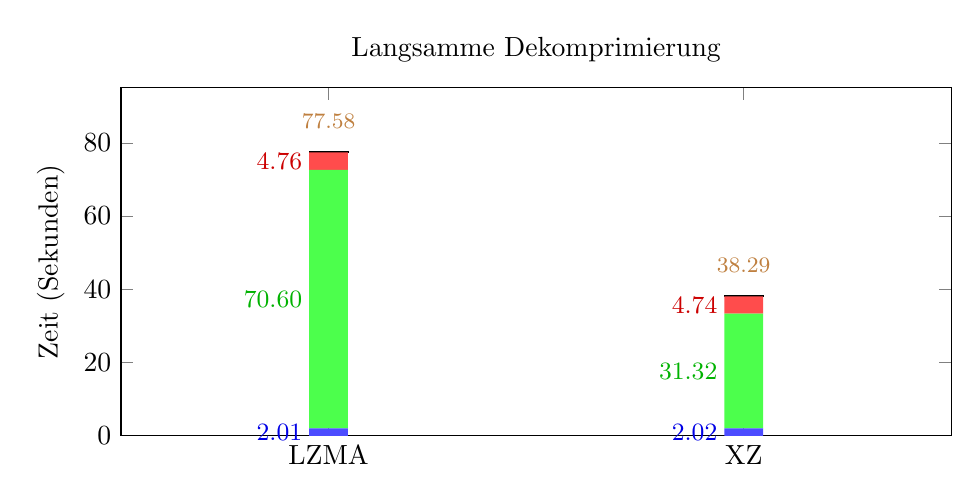
\begin{tikzpicture}
			\begin{axis}[
					ybar stacked,
					bar width=14pt,
					width=\textwidth,
					height=6cm,
					ylabel={Zeit (Sekunden)},
					symbolic x coords={LZMA, XZ},
					xtick=data,
					ymin=0, ymax=95,
					enlarge x limits=0.5,
					title={Langsamme Dekomprimierung},
					nodes near coords,
					nodes near coords style={
							font=\small,
							/pgf/number format/fixed,
							/pgf/number format/precision=2,
							anchor=east,
							xshift=-6pt,
						},
					every node near coord/.append style={
							/pgfplots/point meta=explicit symbolic,
							font=\small,
						},
					point meta=explicit symbolic,
					legend style={at={(0.5,-0.25)}, anchor=north,legend columns=-1,font=\small}
				]
				% U-Boot Time (blue)
				\addplot+[fill=blue!70, draw=none, nodes near coords style={text=blue!90!black}]
				coordinates {(LZMA,2.0127)[2.01] (XZ,2.0211)[2.02]};
				% Uncompress Time (green)
				\addplot+[fill=green!70, draw=none, nodes near coords style={text=green!70!black}]
				coordinates {(LZMA,70.5996)[70.60] (XZ,31.3218)[31.32]};
				% Kernel Time (red)
				\addplot+[fill=red!70, draw=none, nodes near coords style={text=red!80!black}]
				coordinates {(LZMA,4.7573)[4.76] (XZ,4.7414)[4.74]};
				\addplot+[
					nodes near coords={
							\textbf{\textcolor{brown}{\pgfmathprintnumber[fixed,precision=2]{\pgfplotspointmeta}}}
						},
					nodes near coords style={
							anchor=south,
							yshift=5pt,
							xshift=6pt,
							font=\footnotesize\bfseries
						},
					point meta={y}
				]
				coordinates {
						(LZMA, 0.21)
						(XZ, 0.21)
					};
			\end{axis}
		\end{tikzpicture}
		\vspace{0.5em}
	\end{minipage}
	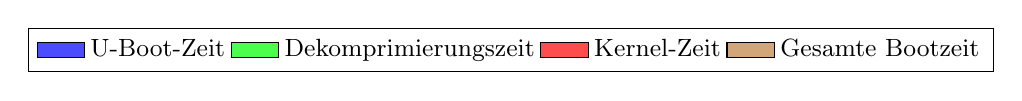
\begin{tikzpicture}
		\begin{axis}[
				hide axis,
				axis lines=none,
				tick style={draw=none},
				xmin=0, xmax=1,
				ymin=0, ymax=1,
				legend style={
						at={(0.5,1)},
						anchor=south,
						legend columns=-1,
						font=\small,
					}
			]
			\addlegendimage{area legend, fill=blue!70}
			\addlegendentry{U-Boot-Zeit}
			\addlegendimage{area legend, fill=green!70}
			\addlegendentry{Dekomprimierungszeit}
			\addlegendimage{area legend, fill=red!70}
			\addlegendentry{Kernel-Zeit}
			\addlegendimage{area legend, fill=brown!70}
			\addlegendentry{Gesamte Bootzeit}
		\end{axis}
	\end{tikzpicture}
	\vspace{-13em}
	\caption{Vergleich der durchschnittlichen Bootzeitkomponenten für schnelle und langsame
		Dekomprimierungsalgorithmen}
	\label{fig:boot_times_split}
\end{figure}


In dem Git-Repository dieser Projektarbeit is auch ein Skript beigefügt, das die Bootzeitmessung
automatisiert, indem es die serielle Konsolenausgabe über eine angegebene serielle Schnittstelle
überwacht~\cite{myBootMeasureScript}. Es extrahiert Zeitstempel aus wichtigen Bootmeldungen, berechnet daraus
die Dauer der einzelnen Phasen und schreibt die Ergebnisse zur späteren Analyse in eine CSV-Datei.


\textbf{Definitionen der gemessenen Bootzeit-Komponenten:}
\begin{itemize}
	\item \textbf{U-Boot-Zeit:} Die Dauer vom Start des Bootvorgangs bis zum Beginn des Linux-Kernels. Dies
	      umfasst die Initialisierung und Konfiguration des Bootloaders. Im Skript entspricht dies der Zeit vom
	      Startzeitstempel bis zur Log-Nachricht „Starting kernel ...“.
	\item \textbf{Dekomprimierungszeit:} Die Zeit, die der Kernel benötigt, um das komprimierte Kernel-Image zu
	      dekomprimieren. Sie beginnt mit der Log-Nachricht „Uncompressing Linux...“ und endet kurz bevor der Kernel
	      die CPU vollständig startet. In dieser Phase beeinflusst die Dekomprimierungsleistung der verschiedenen
	      Komprimierungsmethoden direkt die Bootzeit.
	\item \textbf{Kernel-Zeit:} Der Zeitraum, in dem der Linux-Kernel die Hardware initialisiert, das
	      Root-Dateisystem einhängt und die Benutzerumgebung vorbereitet, bis der Login-Prompt erscheint. Diese
	      Phase reicht vom Start des Kernels bis zum vom Skript erkannten Login-Prompt.
	\item \textbf{Gesamte Bootzeit:} Die gesamte Zeitspanne vom Einschalten oder Zurücksetzen des Systems bis es
	      zur Anmeldung bereit ist. Sie umfasst die U-Boot-Zeit, die Dekomprimierungszeit, die
	      Kernel-Initialisierung und Userscript-Zeit (nicht angegeben).
\end{itemize}

\subsection{Kernelgröße reduzieren}
Eine Reduzierung der Kernelgröße kann die Ladezeiten verbessern. Nicht benötigte Funktionen sollten als Module
kompiliert oder ganz deaktiviert werden. Optionen wie \textit{CONFIG\_KALLSYMS}, \textit{CONFIG\_DEBUG\_FS}
und \textit{CONFIG\_BUG} können abgeschaltet werden, um die Kernelgröße weiter zu verringern. Spezielle
Features für Embedded-Systeme, wie \textit{CONFIG\_EMBEDDED} und \textit{CONFIG\_SLUB\_TINY}, helfen ebenfalls
dabei, den Speicherverbrauch zu minimieren.

\subsection{Weitere Kernel Optimierungen}
Zusätzliche Optimierungen können die Bootzeit weiter verringern. Durch das Kompilieren mit \textit{gcc -Os}
(\textit{CONFIG\_CC\_OPTIMIZE\_FOR\_SIZE}) wird der erzeugte Code kleiner, was die Ladezeiten reduziert.
Verzögerte Initialisierungen von Treibern und \textit{initcall}-Funktionen helfen, den Bootprozess effizienter
zu gestalten. Die Konsolenausgabe kann mit dem Kernelparameter \textit{quiet} deaktiviert werden, um unnötige
Verzögerungen durch Debug-Meldungen zu vermeiden. Zudem kann der Loops-Per-Jiffy-Wert (\textit{lpj})
vorkonfiguriert werden, um das Kalibrieren beim Booten zu überspringen. Auf Systemen mit nur einem Kern sollte
die Multiprozessorunterstützung (\textit{CONFIG\_SMP}) deaktiviert werden, um den Kernel weiter zu
verschlanken. Schließlich kann der Kernel im Thumb2-Modus kompiliert werden (\textit{CONFIG\_THUMB2\_KERNEL}),
was den Code kompakter macht und die Ausführungszeit verkürzen kann.

\begin{figure}[H]
	\centering
	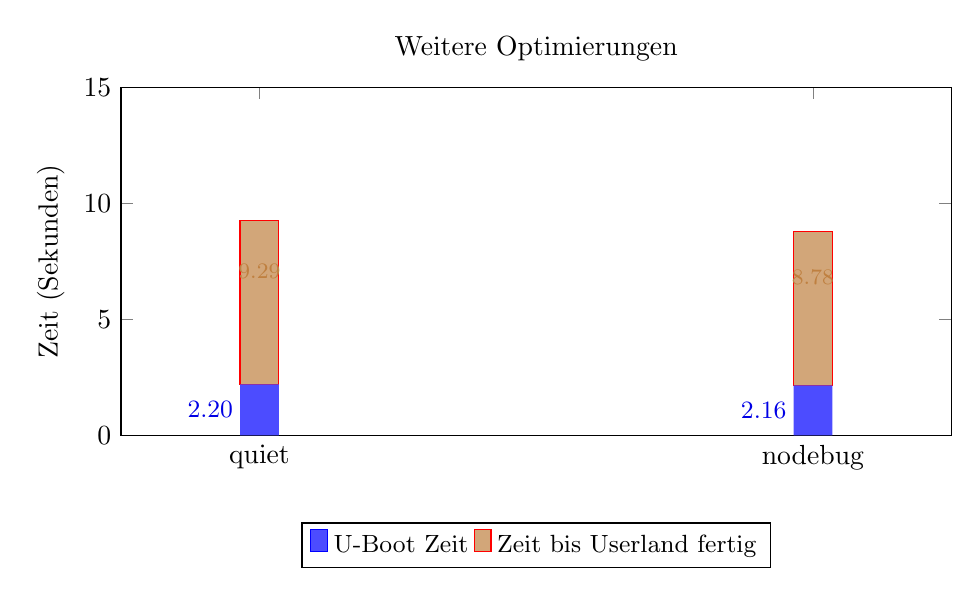
\begin{tikzpicture}
		\begin{axis}[
				ybar stacked,
				bar width=14pt,
				width=\textwidth,
				height=6cm,
				legend style={at={(0.5,-0.25)}, anchor=north,legend columns=-1,font=\small},
				ylabel={Zeit (Sekunden)},
				symbolic x coords={quiet, nodebug},
				xtick=data,
				ymin=0, ymax=15,
				enlarge x limits=0.25,
				title={Weitere Optimierungen},
				nodes near coords,
				nodes near coords style={
						font=\small,
						/pgf/number format/fixed,
						/pgf/number format/precision=2,
						anchor=east,
						xshift=-6pt,
					},
				every node near coord/.append style={
						/pgfplots/point meta=explicit symbolic,
						font=\small,
					},
				point meta=explicit symbolic,
			]
			% U-Boot Time (blue)
			\addplot+[fill=blue!70, draw=none, nodes near coords style={text=blue!90!black}]
			coordinates {(quiet,2.2034)[2.20] (nodebug,2.165217)[2.16] };
			\addlegendentry{U-Boot Zeit}
			\addplot+[
				fill=brown!70,
				nodes near coords={
						\textbf{\textcolor{brown}{\pgfmathprintnumber[fixed,precision=2]{\pgfplotspointmeta}}}
					},
				nodes near coords style={
						text=brown!70!black,
						anchor=south,
						yshift=5pt,
						xshift=6pt,
						font=\footnotesize\bfseries
					},
				point meta={y}
			]
			coordinates {
					(quiet, 7.0841)
					(nodebug, 6.6100)
				};
			\addlegendentry{Zeit bis Userland fertig}
		\end{axis}
	\end{tikzpicture}
\end{figure}

Beide Optimierungen basieren auf der Konfiguration des LZ4-Kompressionsalgorithmus, und können mit diesem
verglichen werden. Die nodebug Konfiguration hat sämtliche Debuging-Optionen aus dem Kernel rauskompeliert,
während die Kernel-Option quiet diese nicht mehr auf der Konsole ausgibt, weshalb nach dem Start des Kernels
bis zurt Login-Promt keine Meldungen mehr angezeigt werden.
